\scanpage{18}

$4$ sommets d'ordre $6$ $+6$ sommets d'ordre $6$ $+12$ sommets d'ordre $3$

$24$ triangles $+4$ hexagones

\figure{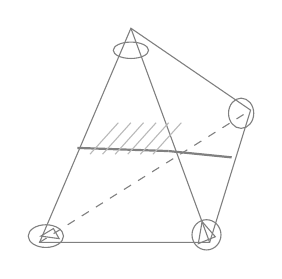
\begin{tikzpicture}[scale=0.8]
\draw[gray] (0,0)--(1.45,3.4)--(3.35,2.1)--(2.7,0)--cycle;
\draw[gray] (1.45,3.4)--(2.7,0);
\draw[dashed,gray] (0,0)--(3.35,2.1);
\draw[gray,thick] (0.6,1.5)--(2.05,1.45);
\draw[gray,thick] (2.05,1.45)--(3.05,1.35);
\draw[gray] (1.45,3.05) ellipse (0.28 and 0.13);
\draw[gray] (0.1,0.1) ellipse (0.28 and 0.18);
\draw[gray] (2.65,0.12) ellipse (0.23 and 0.24);
\draw[gray] (3.2,2.05) ellipse (0.2 and 0.24);
\draw[gray,thin] (0.02,0.1)--(0.22,0.22)--(0.31,0.06)--cycle;
\draw[gray,thin] (2.52,-0.02)--(2.58,0.33)--(2.79,0.09)--cycle;
\foreach \x in {0.8,1,1.2,1.4,1.6,1.8}{\draw[gray!55] (\x,1.4)--(\x+0.45,1.9);}
\end{tikzpicture}}

\figure{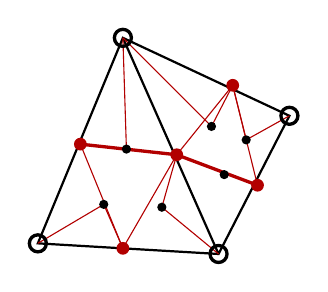
\begin{tikzpicture}[scale=0.9]
\coordinate (A) at (0,0); \coordinate (B) at (1.2,2.9);
\coordinate (C) at (2.55,-0.15); \coordinate (D) at (3.55,1.8);
\draw[thick] (A)--(B)--(D)--(C)--cycle (B)--(C);
\draw[red!70!black,very thick] (0.6,1.4)--(1.96,1.25)--(3.1,0.82);
\draw[red!70!black] (B)--(1.25,1.33) (0.6,1.4)--(1.2,-0.07)--(1.96,1.25)--(2.75,2.23)--(3.1,0.82);
\draw[red!70!black] (A)--(0.93,0.55)--(1.2,-0.07) (C)--(1.75,0.51)--(1.96,1.25);
\draw[red!70!black] (B)--(2.45,1.65)--(2.75,2.23) (D)--(2.94,1.46)--(2.75,2.23);
\foreach \p in {A,B,C,D}{\draw[very thick] (\p) circle (0.12);}
\foreach \p in {(0.6,1.4),(1.96,1.25),(3.1,0.82),(1.2,-0.07),(2.75,2.23)}{\fill[red!70!black] \p circle (0.09);}
\foreach \p in {(1.25,1.33),(0.93,0.55),(1.75,0.51),(2.45,1.65),(2.94,1.46),(2.63,0.97)}{\fill \p circle (0.065);}
\end{tikzpicture}}

\margin{\unsure{voir aussi} cf verso (\unsure{barycentres de} \unsure{triangulation})}

\[
\begin{aligned}
s_0&=4+6+4.3=22\\
s_1&=12+4.\unsure{8|9}=48\\
s_2&=4.7=28
\end{aligned}
\]

\figure{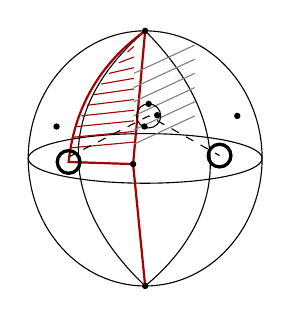
\begin{tikzpicture}[scale=0.9]
\draw (0,0) ellipse (1.65 and 1.8);
\draw (0,0) ellipse (1.65 and 0.35);
\draw (0,1.8) .. controls (-1.45,0.55) and (-1.05,-0.8) .. (0,-1.8);
\draw (0,1.8) .. controls (1.3,0.5) and (1.15,-0.85) .. (0,-1.8);
\draw[red!65!black,thick] (0,1.8)--(-0.17,-0.08)--(0,-1.8);
\draw[red!65!black,thick] (0,1.8) .. controls (-0.8,1.22) and (-1.02,0.5) .. (-1.08,-0.05)--(-0.17,-0.08);
\foreach \y/\x in {0.15/-1.04,0.3/-1.01,0.45/-0.96,0.6/-0.9,0.75/-0.82,0.9/-0.72,1.05/-0.62,1.2/-0.51,1.35/-0.37,1.5/-0.25}{\draw[red!65!black] (\x,\y)--(-0.16,\y+0.08);}
\foreach \y in {0.2,0.4,0.6,0.8,1,1.2}{\draw[gray] (-0.16,\y)--(0.7,\y+0.4);}
\draw[very thick] (-1.08,-0.05) circle (0.16) (1.05,0.04) circle (0.16);
\draw[dashed] (-1.08,0.02)--(0.05,0.6)--(1.05,0.04);
\draw (0.05,0.6) circle (0.17);
\foreach \p in {(0,1.8),(0,-1.8),(-1.25,0.45),(1.3,0.6),(-0.17,-0.08),(0.05,0.77),(0.17,0.61),(-0.01,0.45)}{\fill \p circle (0.045);}
\end{tikzpicture}}

\figure{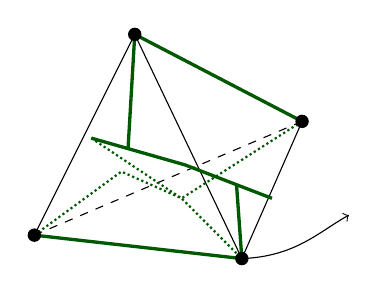
\begin{tikzpicture}[scale=0.85]
\coordinate (A) at (0,0); \coordinate (B) at (1.5,3);
\coordinate (C) at (3.1,-0.35); \coordinate (D) at (4,1.7);
\draw (A)--(B)--(C) (C)--(D);
\draw[green!35!black,very thick] (A)--(C) (B)--(D);
\draw[dashed] (A)--(D);
\draw[green!35!black,very thick] (0.85,1.45)--(2.25,1.05)--(3.55,0.55) (B)--(1.4,1.3) (C)--(3.02,0.76);
\draw[green!35!black,densely dotted,thick] (A)--(1.3,0.95)--(2.2,0.55)--(C);
\draw[green!35!black,densely dotted,thick] (0.85,1.45)--(2.2,0.55)--(D);
\foreach \p in {A,B,C,D}{\fill (\p) circle (0.1);}
\draw[->] (C) .. controls (3.9,-0.32) and (4.25,0.05) .. (4.7,0.3);
\end{tikzpicture}}

\margin{ça fait $2^4-1=15$ \unsure{possibilités} \unsure{d'inversion} \unsure{des faces choisies} \unsure{en} \unsure{des} \unsure{bords} !}

\uline{$4$ types de points-base}

$\bullet$ $3$ structures carrées, sur $I$ (ou $J$)

$\textcolor{red!70!black}{\bullet}$ $2$ structures \unsure{tétraèdres|tétraédriques} $=$ \unsure{orientation des faces}

$\textcolor{red!30!black}{\bullet}$ $6$ structures \inserted{bi}\unsure{pantaloniques} \unsure{appariées|opposées} (maillot ceinturé) (carrée $+$ codiagonale \unsure{$J$} $\simeq$ repère de $J$)

\[
\updownarrow
\]

$\bullet$ $6$ structures pantaloniques de \unsure{quasi-gss} (\unsure{quart de tore})
($\simeq$ carré, $+$ orientation de $I$ i.e. de $J$ $\simeq$ repère de $J$)

\margin{$\omega_I=\unsure{{}^{6J}\omega_J}$}

\diagram{\begin{tikzcd}
\operatorname{rep}(J) \arrow[d,leftrightarrow]\\
J\times\omega_J
\end{tikzcd}}

\figure{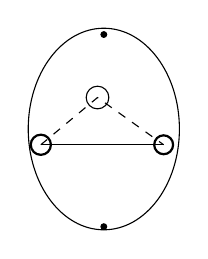
\begin{tikzpicture}[scale=0.8]
\draw (0,0) ellipse (1.2 and 1.6);
\draw (-1,-0.25)--(0.95,-0.25);
\draw[dashed] (-1,-0.25)--(-0.1,0.5)--(0.95,-0.25);
\draw (-0.1,0.5) circle (0.18);
\draw[thick] (-1,-0.25) circle (0.16) (0.95,-0.25) circle (0.15);
\fill (0,1.5) circle (0.055); \fill (0,-1.55) circle (0.055);
\end{tikzpicture}}

\figure{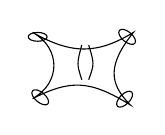
\begin{tikzpicture}[scale=0.8]
\draw (0,0) .. controls (0.45,0.25) and (0.45,0.8) .. (0,1.05)
.. controls (0.65,0.68) and (1.05,0.72) .. (1.6,1.05)
.. controls (1.2,0.55) and (1.2,0.25) .. (1.55,-0.1)
.. controls (0.9,0.3) and (0.6,0.3) .. (0,0);
\draw (0.08,0.98) ellipse (0.15 and 0.07);
\draw[rotate around={-40:(0.12,0.02)}] (0.12,0.02) ellipse (0.16 and 0.08);
\draw[rotate around={-40:(1.5,0.98)}] (1.5,0.98) ellipse (0.16 and 0.08);
\draw[rotate around={45:(1.46,-0.01)}] (1.46,-0.01) ellipse (0.16 and 0.08);
\draw (0.78,0.85)..controls(0.7,0.55)..(0.78,0.3);
\draw (0.89,0.85)..controls(0.98,0.55)..(0.89,0.3);
\end{tikzpicture}}

\margin{sur cette figure, on voit à la fois la \unsure{p.r.q.} du tétraèdre : la configuration-carré, et : la configuration bien \unsure{pantalonnée} du \unsure{quasi-gss}.}

\figure{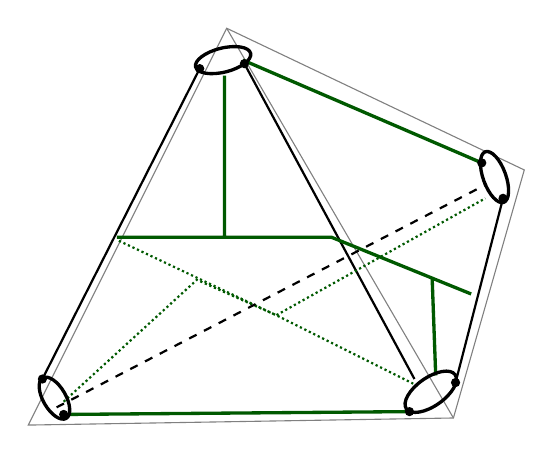
\begin{tikzpicture}[scale=0.9]
\coordinate (A) at (0,0); \coordinate (B) at (2.5,5);
\coordinate (C) at (5.5,0.05); \coordinate (D) at (6.5,3.4);
\draw[thin,gray] (-0.2,-0.15)--(2.6,5.45)--(6.8,3.45)--(5.8,-0.05)--cycle;
\draw[thin,gray] (2.6,5.45)--(5.8,-0.05);
\draw[thick] (0,0.5)--(2.22,4.88) (2.85,4.95)--(5.25,0.5) (5.83,0.45)--(6.5,3.05);
\draw[green!35!black,very thick] (0.32,0)--(5.18,0.04) (2.83,5)--(6.2,3.55);
\draw[green!35!black,very thick] (1.05,2.5)--(4.08,2.5)--(6.05,1.7) (2.57,4.78)--(2.57,2.5) (5.55,0.55)--(5.5,1.92);
\draw[green!35!black,densely dotted,thick] (0.3,0.18)--(2.18,1.9)--(3.3,1.4)--(5.3,0.4);
\draw[green!35!black,densely dotted,thick] (1.08,2.45)--(3.3,1.4)--(6.25,3.05);
\draw[dashed,thick] (0.2,0.1)--(6.27,3.25);
\draw[very thick,rotate around={14:(2.55,5)}] (2.55,5) ellipse (0.4 and 0.17);
\draw[very thick,rotate around={-60:(0.17,0.23)}] (0.17,0.23) ellipse (0.33 and 0.16);
\draw[very thick,rotate around={35:(5.48,0.32)}] (5.48,0.32) ellipse (0.42 and 0.2);
\draw[very thick,rotate around={110:(6.38,3.35)}] (6.38,3.35) ellipse (0.38 and 0.16);
\foreach \p in {(0,0.5),(0.3,0),(2.22,4.88),(2.85,4.95),(5.18,0.04),(5.83,0.45),(6.2,3.55),(6.5,3.05)}{\fill \p circle (0.065);}
\end{tikzpicture}}

\uline{$4$ types de chemins élémentaires}$^{*}$

a) ``\unsure{quart de} twist'' $(2\times3\times4)$ (contour d'un trou)

b) ``sixième de tour'' $(2\times2\times3)$ (sur équateur)

c) pôle vers trou $(2\times2\times3)$ et inv.

d) pôle vers équateur et inv. $(2\times2\times3)$

$2$ types composés supplém.

e) trou vers trou $(2\times3)$ ou ``tiers de tour''

f) demi twist $(2\times2\times3)$

[et bien sûr, g) twist complet $2\times2\times3)$]

\uline{relations} ...

\figure{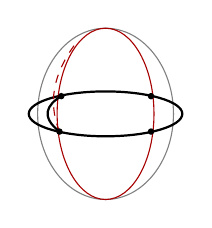
\begin{tikzpicture}[scale=0.75]
\draw[gray] (0,0) ellipse (1.15 and 1.45);
\draw[thick] (0,0) ellipse (1.3 and 0.38);
\draw[red!65!black] (0,0) ellipse (0.82 and 1.45);
\draw[red!65!black,dashed] (-0.78,-0.3)..controls(-1.02,0.3)and(-0.8,0.8)..(-0.5,1.2);
\draw[thick] (-0.78,-0.3)..controls(-1.1,-0.05)and(-1,0.15)..(-0.75,0.3);
\foreach \p in {(-0.78,-0.3),(-0.75,0.3),(0.77,-0.3),(0.77,0.3)}{\fill \p circle (0.055);}
\end{tikzpicture}}

\margin{17}

\margin{$*$ avec les deux sens de parcours, cela fait \uline{huit} types de déformations, à visualiser a) du pt de vue conforme b) du pt de vue combinatoire (ici encore deux pts de vue possibles)}
